\documentclass{article}
\usepackage[utf8]{inputenc}
\usepackage{hyperref}
\usepackage[letterpaper, portrait, margin=1in]{geometry}
\usepackage{enumitem}
\usepackage{amsmath}
\usepackage{booktabs}
\usepackage{graphicx}
\usepackage{amsmath}

\usepackage{hyperref}
\hypersetup{
colorlinks=true,
    linkcolor=black,
    filecolor=black,      
    urlcolor=blue,
    citecolor=black,
}
\usepackage{natbib}

\usepackage{titlesec}
\titleformat{\section}
{\normalfont\Large\bfseries}{\thesection}{1em}{}[{\titlerule[0.8pt]}]


\title{ECON7103HW4}
\author{Sedat Ors}
\date{13 February 2023}

\begin{document}

\maketitle

\section{Python}
\vspace{0.5cm}
\begin{enumerate}
\item 
\noindent According to the Figure 1, there are parallel trends before treatment. 

\begin{figure}[]
    \centering
     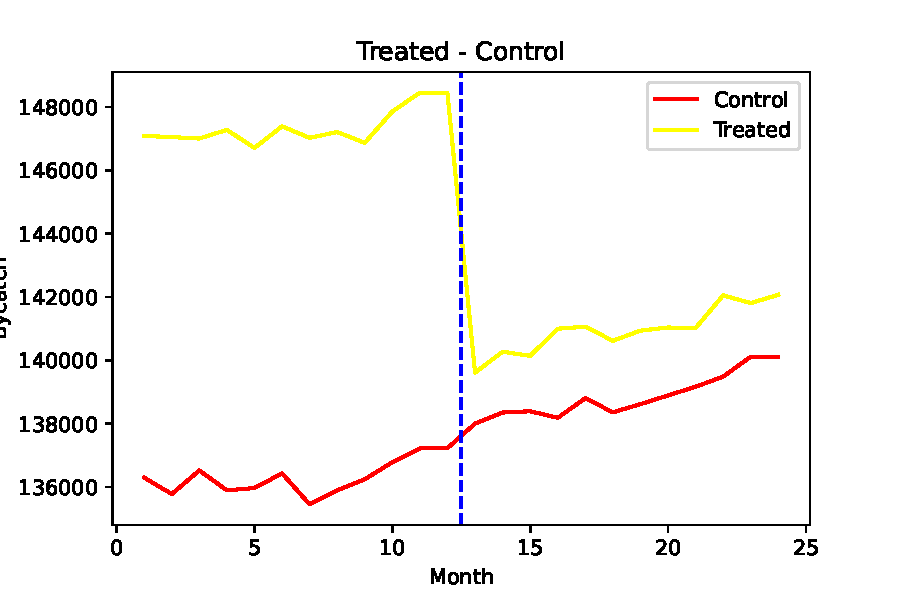
\includegraphics{hw4Q1.pdf}
    \caption{}
    \label{tab:question3}
\end{figure}


\item The estimation is -9,591 which means that treatment leads decline in treatment group. 

\item
\noindent See Table 1 for results.
\vspace{0.5cm}
\begin{table}[]
    \centering
    \begin{tabular}{llll}
\toprule
{} &                     (1) &                    (2) &                   (3) \\
\midrule
Alpha           &               138001.81 &                    NaN &                   NaN \\
                &  (100507.57, 175496.06) &                    NaN &                   NaN \\
Pre period      &                 -773.22 &                    NaN &                   NaN \\
                &      (-1976.32, 429.89) &                    NaN &                   NaN \\
Treatment       &                11202.04 &                    NaN &                   NaN \\
                &   (-36028.81, 58432.89) &                    NaN &                   NaN \\
Time Treated    &                -9591.35 &                    NaN &                   NaN \\
                &   (-16085.87, -3096.83) &                    NaN &                   NaN \\
After-treatment &                   100.0 &                    NaN &                   NaN \\
Alpha           &                     NaN &              132088.04 &                   NaN \\
                &                     NaN &   (96407.7, 167768.38) &                   NaN \\
Treatment       &                     NaN &               11052.45 &                   NaN \\
                &                     NaN &  (-35515.12, 57620.02) &                   NaN \\
Time Treated    &                     NaN &               -8956.78 &                   NaN \\
                &                     NaN &  (-15323.66, -2589.91) &                   NaN \\
dummy           &                     NaN &                4066.01 &                   NaN \\
                &                     NaN &      (2681.31, 5450.7) &                   NaN \\
dummy           &                     NaN &                 3808.7 &                   NaN \\
                &                     NaN &     (2623.31, 4994.08) &                   NaN \\
dummy           &                     NaN &                4127.06 &                   NaN \\
                &                     NaN &     (2663.81, 5590.32) &                   NaN \\
dummy           &                     NaN &                3984.54 &                   NaN \\
                &                     NaN &     (2478.29, 5490.79) &                   NaN \\
dummy           &                     NaN &                3710.72 &                   NaN \\
                &                     NaN &     (2438.58, 4982.86) &                   NaN \\
dummy           &                     NaN &                4292.12 &                   NaN \\
                &                     NaN &     (3061.12, 5523.12) &                   NaN \\
dummy           &                     NaN &                3644.76 &                   NaN \\
                &                     NaN &      (2349.3, 4940.22) &                   NaN \\
dummy           &                     NaN &                 3950.1 &                   NaN \\
                &                     NaN &     (2723.76, 5176.45) &                   NaN \\
dummy           &                     NaN &                3925.03 &                   NaN \\
                &                     NaN &     (2665.91, 5184.16) &                   NaN \\
dummy           &                     NaN &                4705.95 &                   NaN \\
                &                     NaN &     (3420.39, 5991.51) &                   NaN \\
dummy           &                     NaN &                5229.24 &                   NaN \\
                &                     NaN &     (3756.13, 6702.35) &                   NaN \\
dummy           &                     NaN &                5221.34 &                   NaN \\
                &                     NaN &     (3735.33, 6707.34) &                   NaN \\
dummy           &                     NaN &                5651.89 &                   NaN \\
                &                     NaN &     (3804.73, 7499.05) &                   NaN \\
dummy           &                     NaN &                6169.52 &                   NaN \\
                &                     NaN &     (4277.39, 8061.65) &                   NaN \\
dummy           &                     NaN &                6116.86 &                   NaN \\
                &                     NaN &      (4296.1, 7937.63) &                   NaN \\
dummy           &                     NaN &                6485.46 &                   NaN \\
                &                     NaN &     (4617.13, 8353.79) &                   NaN \\
dummy           &                     NaN &                6803.65 &                   NaN \\
                &                     NaN &     (4956.31, 8650.98) &                   NaN \\
dummy           &                     NaN &                6359.83 &                   NaN \\
                &                     NaN &      (4569.16, 8150.5) &                   NaN \\
dummy           &                     NaN &                6650.62 &                   NaN \\
                &                     NaN &     (4763.69, 8537.56) &                   NaN \\
dummy           &                     NaN &                6830.44 &                   NaN \\
                &                     NaN &     (4956.02, 8704.85) &                   NaN \\
dummy           &                     NaN &                6946.89 &                   NaN \\
                &                     NaN &     (4924.74, 8969.04) &                   NaN \\
dummy           &                     NaN &                 7652.8 &                   NaN \\
                &                     NaN &     (5669.86, 9635.74) &                   NaN \\
dummy           &                     NaN &                7809.03 &                   NaN \\
                &                     NaN &     (5751.81, 9866.26) &                   NaN \\
dummy           &                     NaN &                7945.49 &                   NaN \\
                &                     NaN &    (5845.15, 10045.82) &                   NaN \\
After-Treatment &                     NaN &                 1200.0 &                   NaN \\
Alpha           &                     NaN &                    NaN &               1547.01 \\
                &                     NaN &                    NaN &    (-675.23, 3769.24) \\
Treatment       &                     NaN &                    NaN &                 -21.9 \\
                &                     NaN &                    NaN &     (-641.34, 597.54) \\
Time Treated    &                     NaN &                    NaN &              -8436.28 \\
                &                     NaN &                    NaN &  (-14111.27, -2761.3) \\
shrimp          &                     NaN &                    NaN &                  1.06 \\
                &                     NaN &                    NaN &          (0.95, 1.16) \\
salmon          &                     NaN &                    NaN &                   0.6 \\
                &                     NaN &                    NaN &          (0.18, 1.02) \\
firmsize        &                     NaN &                    NaN &              -2119.71 \\
                &                     NaN &                    NaN &   (-8966.26, 4726.83) \\
dummy           &                     NaN &                    NaN &                 15.77 \\
                &                     NaN &                    NaN &       (-31.68, 63.22) \\
dummy           &                     NaN &                    NaN &                -15.41 \\
                &                     NaN &                    NaN &       (-92.78, 61.96) \\
dummy           &                     NaN &                    NaN &                -11.21 \\
                &                     NaN &                    NaN &     (-136.49, 114.07) \\
dummy           &                     NaN &                    NaN &                 -4.04 \\
                &                     NaN &                    NaN &     (-149.39, 141.31) \\
dummy           &                     NaN &                    NaN &                -55.75 \\
                &                     NaN &                    NaN &     (-313.27, 201.77) \\
dummy           &                     NaN &                    NaN &                -18.03 \\
                &                     NaN &                    NaN &     (-254.12, 218.07) \\
dummy           &                     NaN &                    NaN &                 -55.6 \\
                &                     NaN &                    NaN &     (-388.27, 277.07) \\
dummy           &                     NaN &                    NaN &                -58.87 \\
                &                     NaN &                    NaN &     (-414.48, 296.74) \\
dummy           &                     NaN &                    NaN &               -100.35 \\
                &                     NaN &                    NaN &     (-496.11, 295.41) \\
dummy           &                     NaN &                    NaN &               -139.48 \\
                &                     NaN &                    NaN &      (-638.96, 360.0) \\
dummy           &                     NaN &                    NaN &               -143.76 \\
                &                     NaN &                    NaN &     (-655.53, 368.01) \\
dummy           &                     NaN &                    NaN &               -122.84 \\
                &                     NaN &                    NaN &      (-696.5, 450.83) \\
dummy           &                     NaN &                    NaN &               -188.63 \\
                &                     NaN &                    NaN &      (-857.9, 480.64) \\
dummy           &                     NaN &                    NaN &               -158.76 \\
                &                     NaN &                    NaN &     (-853.38, 535.85) \\
dummy           &                     NaN &                    NaN &               -251.21 \\
                &                     NaN &                    NaN &     (-947.35, 444.92) \\
dummy           &                     NaN &                    NaN &               -265.55 \\
                &                     NaN &                    NaN &      (-1050.1, 519.0) \\
dummy           &                     NaN &                    NaN &                -187.4 \\
                &                     NaN &                    NaN &     (-978.99, 604.19) \\
dummy           &                     NaN &                    NaN &               -271.16 \\
                &                     NaN &                    NaN &     (-1123.41, 581.1) \\
dummy           &                     NaN &                    NaN &               -316.44 \\
                &                     NaN &                    NaN &     (-1229.2, 596.33) \\
dummy           &                     NaN &                    NaN &                -285.1 \\
                &                     NaN &                    NaN &    (-1225.17, 654.97) \\
dummy           &                     NaN &                    NaN &               -377.15 \\
                &                     NaN &                    NaN &    (-1478.18, 723.89) \\
dummy           &                     NaN &                    NaN &                -449.5 \\
                &                     NaN &                    NaN &    (-1568.82, 669.83) \\
dummy           &                     NaN &                    NaN &                -408.7 \\
                &                     NaN &                    NaN &    (-1486.64, 669.23) \\
After Treatment &                     NaN &                    NaN &                1200.0 \\
\bottomrule
\end{tabular}

    \caption{Regression results with heteroskedasticity-robust standard errors.}
    \label{tab:question3}
\end{table}


\end{enumerate}

\section{Stata}
\vspace{0.5cm}
\begin{enumerate}
\item
\noindent See Table 2 for results.
\begin{table}[]
    \centering
    \input{table3}
    \caption{}
\end{table}

\end{enumerate}

\end{document}
